%%%%%%%%%%%%
%
% $Autor: Wings $
% $Datum: 2019-03-05 08:03:15Z $
% $Pfad: SensorDHT22.tex $
% $Version: 4250 $
% !TeX spellcheck = en_GB/de_DE
% !TeX encoding = utf8
% !TeX root = filename 
% !TeX TXS-program:bibliography = txs:///biber
%
%%%%%%%%%%%%

\chapter{Sensor DEBO DHT22 }

Der Sensor DEBO DHT22 wird verwendet, um den fehlenden Sensor im Arduino Nano 33 BLE Sense Lite auszugleichen. Der DHT22 Sensor ermittelt die Temperatur und Luftfeuchtigkeit. Angeschlossen wird der Sensor mit einem 4.7KOhm Pull-Up Widerstand. Angeschlossen wird der Sensor mit Steckbrückenkabel, welche in einen Grovestecker übergehen und mit dem TMLS verbunden sind. Er verfügt über die Anschlüsse GND für die Masse, VCC zur Spannungsversorgung und einen Datenpin zur Datenübertragung. Der Widerstand wird parallel zum Sensor geschaltet.

\begin{center}
    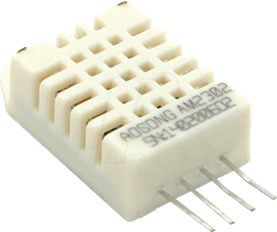
\includegraphics[width=3cm]{Sensor/DHT22/DHT22.png}
    
    \captionof{figure}{Sensor DHT22}
\end{center} 


\section{Luftdruck}

Der Luftdruck wird durch einen ultrakompakten piezoresistiven Absolutdrucksensor ermittelt. Für die elektronische Druckmessung ist ein Sensor erforderlich, der den zu messenden absoluten Luftdruck aufnimmt und in ein elektrisches Signal umwandelt. Unterschieden wird hier zwischen der resistiven und piezoresistiven Druckmessung. 

\subsection{Resistive Druckmessung}

Die resistive Druckmessung ist die klassische Druckmessung und funktioniert über einen dünnen Metallstreifen, dessen Widerstandswert sich bei Verformung ändert. Bei Dehnung wird der Streifen länger und dünner, sodass der elektrische Widerstand steigt. Umgekehrt folgt daraus, dass bei Stauchung der Streifen kürzer wird und der Querschnitt steigt, was wiederum einen verringerten Widerstand aufweist. Um den zu messenden Druck in eine Kontrollierte mechanische Verformung zu Übersetzen, wird der Dehnungsmessstreifen (DMS) auf eine elastische Membran mittels Klebstoff aufgebracht. 
Wirkt nun auf einer Seite dieser Membran ein Überdruck, so verformt sich diese und führt je nach Position zur Stauchung oder Dehnung des DMS, siehe \ref{fig:DMS}.

\begin{figure}[H]	
    \centering
\begin{tikzpicture}[scale=1.0]
    \tikzstyle{every node}=[font=\LARGE]
    
    % Vertikale und horizontale Linien
    \draw (2.25,10.75) -- (2.25,7.5);
    \draw (2.25,7.5) -- (3.25,7.5);
    \draw (3.25,7.5) -- (3.25,10.25);
    \draw (3.25,10.25) -- (6.25,10.25);
    \draw (6.25,10.25) -- (6.25,7.5);
    \draw (6.25,7.5) -- (7.25,7.5);
    \draw (7.25,7.5) -- (7.25,11);
    \draw (7.25,11) -- (2.25,11);
    \draw (2.25,11) -- (2.25,10.75);
    
    % Zusätzliche Linien
    \draw (4.75,11) -- (4.75,11.25);
    \draw (4.75,11.25) -- (5.25,11.25);
    \draw (5.25,11.25) -- (5.25,11);
    \draw (6,11) -- (6,11.25);
    \draw (6,11.25) -- (6.5,11.25);
    \draw (6.5,11.25) -- (6.5,11);
    \draw (5,11.75) -- (6.5,12.5);
    \draw (6.25,11.5) -- (6.5,12.5);
    % Beschriftung
    \node[align=center, anchor=south, font=\small] at (8.4, 12.4) {Dehnungsmessstreifen};
\end{tikzpicture}
    \caption{Positionierung der DMS auf Membran}
    \label{fig:DMS}
\end{figure}

\subsection{Piezorestistive Druckmessung}

Die piezorestistive Druckmessung basiert auf einem ähnlichem Prinzip. Auch hier bewirkt eine Verlängerung oder Verkürzung eine Änderung des Widerstandes. Zusätzlich führt in einem piezorestiven Material die mechanische Spannung, die bei Dehnung oder Stauchung auftritt, auch zu einer Änderung der elektrischen Leitfähigkeit. Dieser Effekt basiert auf Verschiebungen der Atompositionen zueinander, welche sich direkt auf den elektrischen Ladungstransport auswirken. Die aus der Änderung der elektrischen Leitfähigkeit resultierende Widerstandsänderung kann deutlich größer ausfallen als jene, die durch reine Verformung bedingt ist. Grundlage für einen piezoresistiven Sensorchip sind weniger als einen Millimeter dünne, kristalline Siliziumscheiben, sogenannte Wafer. In dessen Oberfläche werden an bestimmten Stellen Fremdatome eingebracht, die örtlich gezielt die Leitfähigkeit beeinflussen. Dieser Prozess ist das sogenannte Dotieren, und diese dotierten Gebiete im Silizium bilden die piezoresistiven Widerstände. 

In einem nachfolgenden Prozessschritt wird dann das Siliziumwafer örtlich so abgedünnt, dass Membranen direkt im Silizium entstehen und die piezoresistiven Widerstände, ähnlich wie in \ref{fig:DMS} gezeigt, an bestimmen Positionen liegen. Wirkt nun auf eine Seite dieser Membran ein Druck, verformt sich diese und bewirkt so eine mechanische Spannung in den piezoresistiven Widerständen. Je nach Position nimmt der Widerstandswert zu oder ab. Über die Dicke der verbleibenden Membran lässt sich die Druckempfindlichkeit des Sensorchips einstellen. Anschließend wird die Rückseite des Siliziums fest mit einem Glas verbunden, siehe \ref{fig:PIEZO}. Dabei entsteht für Absolutdrucksensoren ein abgeschlossener Referenzraum unter Vakuum. Für die Messung eines Relativdrucks enthält das rückseitige Glas ein Referenzloch.

\begin{figure}[H]	
    \centering
    
%\usetikzlibrary {arrows.meta}

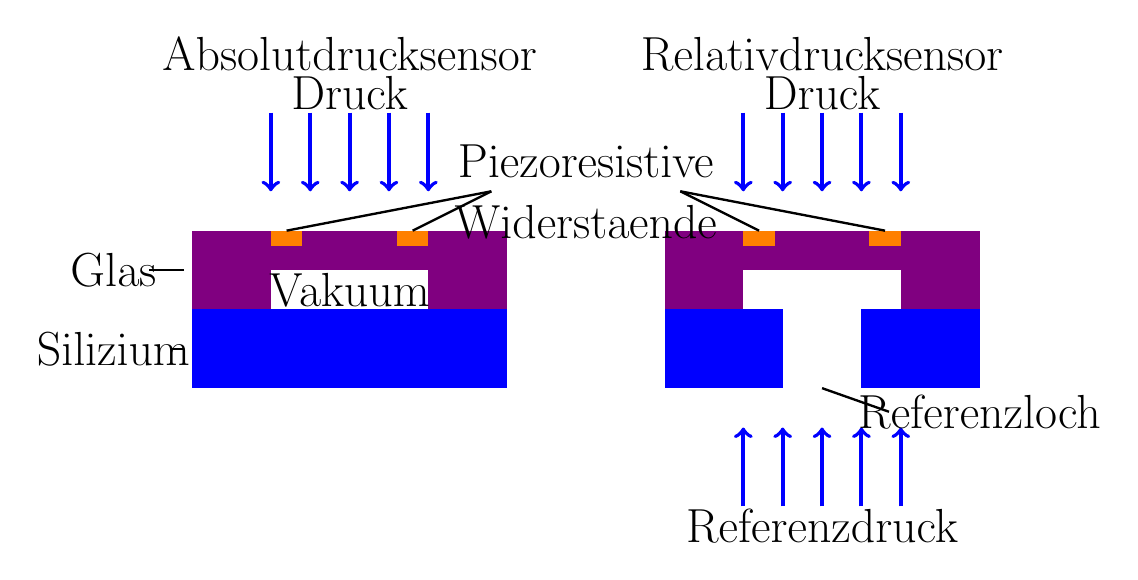
\begin{tikzpicture}
    % Absolutdrucksensor:
    
    % Zeichnen der Rechtecke
    \fill [blue] (0,0) rectangle ++(4,1);
    \fill [violet] (0,1) rectangle ++(4,1);
    \fill [white] (1,1) rectangle ++(2,0.5);
    \fill [orange] (1,2) rectangle ++(0.4,-0.2);
    \fill [orange] (3,2) rectangle ++(-0.4,-0.2);
    
    % Zeichnen der Beschriftungslinien
    \draw [black, line width=0.3mm] (-0.1,0.5) -- (-0.25,0.5);
    \draw [black, line width=0.3mm] (-0.1,1.5) -- (-0.55,1.5);
    
    % Zeichnen der Pfeile
    \foreach \i in {0,1,...,4}
    {
        \draw[blue, line width=0.5mm,->] ({1+\i*0.5},3.5) -- +(0,-1);
    }
    
    % Einfuegen der Beschriftungen
    \draw   (2,1.25) node {Vakuum}
    (2,3.75) node {Druck}
    (-1,0.5) node {Silizium}
    (-1,1.5) node {Glas}
    [font=\bfseries](2,4.25) node {Absolutdrucksensor};
    
    %%%%%%%%%%%%%%%%%%%%%%%%%%%%%%%%%%%%%%%%%%%%%%%%%%%%%%%%%%%%%%%%%%%%%%%%%%%%%%%%%%%%%
    % Relativdrucksensor:
    
    % Zeichnen der Rechtecke
    \fill [blue] (6,0) rectangle ++(4,1);
    \fill [violet] (6,1) rectangle ++(4,1);
    \fill [white] (7,1) rectangle ++(2,0.5);
    \fill [white] (7.5,0) rectangle ++(1,1);
    \fill [orange] (7,2) rectangle ++(0.4,-0.2);
    \fill [orange] (9,2) rectangle ++(-0.4,-0.2);
    
    % Zeichnen der Beschriftungslinien
    \draw [black, line width=0.3mm] (8,0) -- (8.85,-0.3);
    
    \draw [black, line width=0.3mm] (1.2,2) -- (3.8,2.5);
    \draw [black, line width=0.3mm] (2.8,2) -- (3.8,2.5);
    \draw [black, line width=0.3mm] (7.2,2) -- (6.2,2.5);
    \draw [black, line width=0.3mm] (8.8,2) -- (6.2,2.5);
    
    % Zeichnen der Pfeile
    \foreach \i in {0,1,...,4}
    {
        \draw[blue, line width=0.5mm,->] ({7+\i*0.5},3.5) -- +(0,-1);
        \draw[blue, line width=0.5mm,->] ({7+\i*0.5},-1.5) -- +(0,1);
    }
    
    % Einfuegen der Beschriftungen
    \draw   (8,3.75) node {Druck}
    (8,-1.75) node {Referenzdruck}
    (10,-0.3) node {Referenzloch}
    [align=center](5,2.5) node {Piezoresistive \\ Widerstaende}
    [font=\bfseries](8,4.25) node {Relativdrucksensor};
    
\end{tikzpicture}
    \caption{Aufbau des piezoresistiven Sensorchips}
    \label{fig:PIEZO}
\end{figure}

Bei piezoresistiven Druckmesszellen sind die Messwiderstände also im Gegensatz zum DMS in die Membran integriert. Bei dieser Technologie entfällt somit das Aufkleben, was eine wichtige Voraussetzung für Alterungs- und Temperaturbeständigkeit sowie Hysteresefreiheit (Hysterese = Nachwirkung des vorherigen Verformungszustands) ist. Das piezoresistive Messprinzip wird auch in dem DHT22-Sensor verwendet, was zu guten und genauen Messwerten führt \cite{Keller:2019}.

\section{Temperatur}

Die Temperaturmessung kann auf unterschiedliche Weise Erfolgen. Die verbreitetste ist das Flüssigkeitsthermometer, welches aus einem Vorratsgefäß und einem angeschlossenen Steigrohr, auch Kapillare genannt, besteht. Das Vorratsgefäß ist mit einer thermometrischen Flüssigkeit gefüllt, welche sich bei steigender Temperatur ausdehnt und das Steigrohr füllt.

Als alternative Möglichkeiten werden NTC- und PTC-Thermistoren verwendet. Auch genannt Heißleiter und Kaltleiter. Der NTC-Thermistor ist ein variabler elektrischer, wärmeempfindliche Widerstand, dessen Wert sich mit der Temperatur reproduzierbar ändert. Die Widerstände sind nicht linear und der Widerstand nimmt bei steigender Temperatur ab. Die Art und Weise, wie der Widerstand abnimmt, hängt mit einer Konstante zusammen, welche in der Elektroindustrie als Beta bekannt ist. Beta wird in Kelvin gemessen. Ein NTC ist also ein elektronisches Bauteil, welches den Widerstand temperaturabhängig verändert. Diese elektrischen Signale können dann Aufschluss über die Temperatur geben. Der PCT funktioniert vom Prinzip her gleich, jedoch steigt der Widerstand mit zunehmender Temperatur.

Leider wurde auf keiner Seite und in keinem Datenblatt veröffentlicht, um welches Prinzip es sich beim DHT22-Sensor handelt. Jedoch wurde nach der Recherche angenommen, dass ein NTC-Thermistor verbaut ist.  Dies wird dadurch begründet, dass keine Flüssigkeit im Sensor ist, und somit die erste Möglichkeit entfällt. Die Entscheidung gegen den PTC-Thermistor wurde getroffen, da PTC-Thermistoren Verhältnismäßig sehr teuer sind, und da der Sensor gerade einmal 7€ kostet, es sehr unwahrscheinlich ist, dass das Prinzip des PTC verwendet wurde \cite{Ametherm:2024}.

\section{Feuchtigkeit}

Es gibt vier Arten von Feuchtigkeitssensoren, die auf den Funktionsprinzipien und Sensormaterialien basieren: Kapazitiv, resistiv, Wärmeleitfähigkeit, psychometrisch. 

\subsection{Kapazitive Feuchtigkeitssensoren}

Kapazitive Feuchtigkeitssensoren gehören zu den am häufigsten verwendeten Arten. Dieses Prinzip ist auch im DHT22-Sensor verbaut. Die Sensoren funktionieren, indem sie Änderungen der Dielektrizitätskonstante eines Materials als Reaktion auf Änderung der Luftfeuchtigkeit messen. Die Dielektrizitätskonstante  misst die Fähigkeit eines Materials, elektrische Energie in einem elektrischen Feld zu speichern. 

Sie bestehen aus zwei Elektronen, wovon eins mit hygroskopischen Material beschichtet ist, dass Wasserdampf aus der Luft absorbiert. Wenn das hygroskopische Material Wasserdampf aufnimmt, führt dies zu einer Änderung der Dielektrizitätskonstante zwischen den beiden Elektroden, die vom Sensor gemessen wird. 

\subsection{Resistive Feuchtigkeitssensoren}

Resistive Feuchtigkeitssensoren, auch Hygrometer genannt, messen Änderungen im elektrischen Widerstand eines Materials als Reaktion auf der Änderung der Luftfeuchtigkeit. Die gebräuchlichste Art von Widerstandsfeuchtigkeitssensoren ist der polymerbasierte Sensor, welcher aus einem leitfähigen Polymerfilm besteht, der seinen Widerstand ändert, wenn er Wasserdampf ausgesetzt wird. 

Wenn der Polymerfilm Wasserdampf aus der Luft aufnimmt, schwillt er an und wird leitfähiger, wodurch der durch den Sensor fließende elektrische Strom zunimmt. Die Widerstandsänderung ist proportional zur Wasserdampfmenge in der Luft und kann zur Bestimmung der Luftfeuchtigkeit gemessen werden. Dieser Sensortyp ist auch in dem DHT22-Sensor verbaut und basiert auf diesem System. 

\subsection{Wärmeleitfähigkeits Feuchtigkeitssensor}

Wärmeleitfähigkeits-Feuchtigkeitssensoren messen die Wärmeleitfähigkeit eines Gasgemisches als Reaktion auf Änderungen der Luftfeuchtigkeit.Sie bestehen aus einem beheizten Sensorelement und einem Temperatursensor, der den Temperaturunterschied zwischen den Beiden misst. Wenn das Sensorelement Wasserdampf absorbiert, verringert es seine Wärmeleitfähigkeit, was zu einer Temperaturänderung führt, die der Temperatursensor messen kann. Diese Temperaturänderung ist proportional zur Menge an Wasserdampf in der Luft und kann zur Bestimmung der Luftfeuchtigkeit verwendet werden.

\subsection{Psychrometrische Feuchtigkeitssensoren}

Psychrometrische Feuchtigkeitssensoren, auch Taupunktspiegelsensoren genannt, messen die Temperatur, bei der Wasserdampf auf einer Oberfläche kondensiert.Sie bestehen aus einem gekühlten Spiegel, bis sich auf seiner Oberfläche Tau oder Reif bildet. Die Temperatur, bei der diese Kondensation auftritt, ist eine Funktion der relativen Luftfeuchtigkeit der Luft um den Spiegel \cite {Hengko:2024}.


\section{Sensor DHT22}

Der extern angeschlossene Sensor DHT22 ist für die Temperatur- und Luftfeuchtigkeitsmessung verantwortlich. Für den Betrieb wird die Bibliothek \FILE{DHT.h} benötigt, welche von Adafruit angeboten wird. Sie ermöglicht das starten und stoppen des Sensors, sowie das Auslesen der Temperatur und der Luftfeuchtigkeit. Die Bibliothek ist geeignet für die Sensoren vom Type DHT11 und DHT22.

\section{Schaltplan}

\begin{figure}[H]
    \begin{flushleft} 
        \centering
        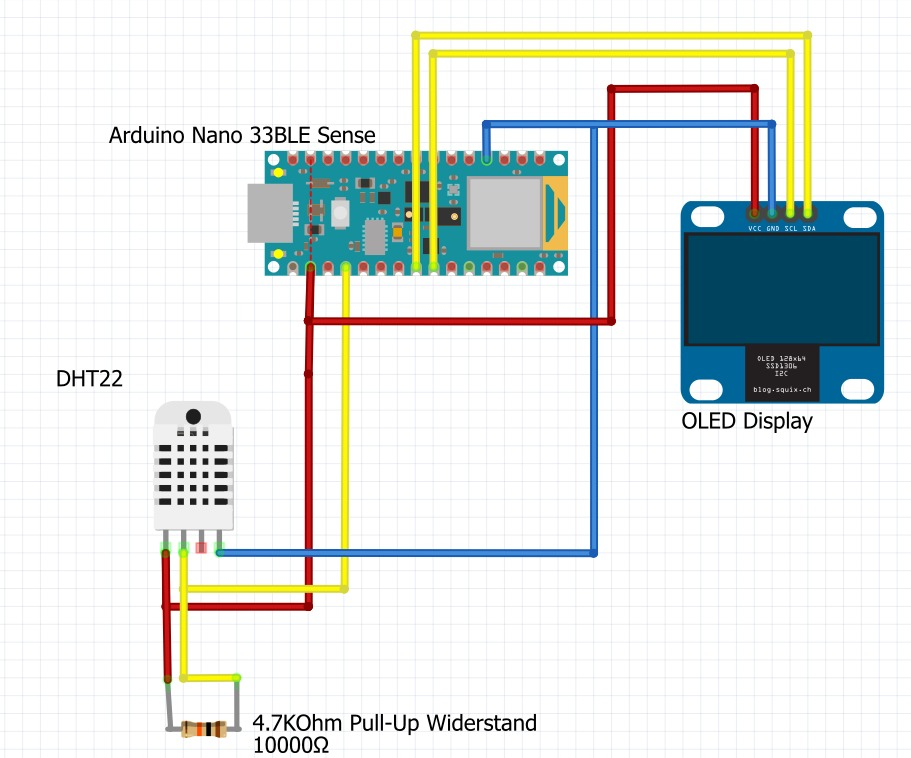
\includegraphics[width=12cm]{Sensor/DHT22/Schaltplan.jpeg}
        \caption{Schaltplan des Raumklimamessgeraets}
        \label{fig:SP}
    \end{flushleft}
\end{figure}


\section{Testen des Sensors  DHT22}

Um die Funktion des LPS22HB-Sensors zu gewährleisten, wurde dieser an den Arduino angeschlossen und mit dem folgenden Programm getestet. Die gemessenen Werte werden seriell an den Computer weitergegeben und im Serial Monitor in der Arduino IDE angezeigt. Dieses Programm wurde zudem zur Kalibrierung verwendet.

\begin{lstlisting}[language=Arduino]
    // Einbinden von verwendeten Bibliotheken
    #include <DHT.h>
    
    // Einstellen des DHT22-Sensors
    #define DHTPIN D11   
    #define DHTTYPE DHT22    
    DHT dht(DHTPIN, DHTTYPE);
    
    void setup() {
        // Einschalten des Sensors
        pinMode(DHTPIN, INPUT);
        dht.begin();
    }
    
    void loop() {
        // Einstellen der Verzoegerung zwischen den Messvorgaengen
        delay(5000);
        
        // Auslesen der Messwerte durch den Sensor
        float humidity = dht.readHumidity(); 
        float temp = dht.readTemperature(); 
        
        // Messwerte seriell ausgeben
        Serial.print("Luftfeuchte: ");
        Serial.println(humidity);
        Serial.println();
        
        Serial.print("Temperatur: ");
        Serial.println(temp);
        Serial.println();
    }
\end{lstlisting}





\section{Kalibrierung}

\subsection{Opus20 THI} 

Das Opus 20 THI ist ein hochpräziser LAN-Datenlogger, der speziell zur Überwachung des Gebäudeklimas und zur Kontrolle klimasensitiver Produktionsprozesse entwickelt wurde. Es wird in EDV-Rechenzentren, Schaltschränken, Windturbinen, Lagerräumen und Museen eingesetzt. Das Gerät zeichnet sich durch seine Genauigkeit, Zuverlässigkeit und einfache Bedienung aus, siehe \ref{fig:Opus20THI}.

\begin{figure}[H]
    \centering
    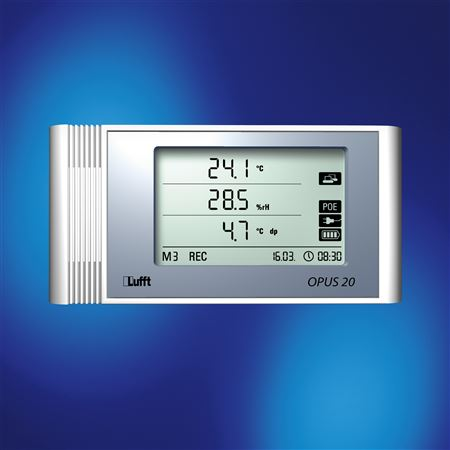
\includegraphics[width=9cm]{Sensor/DHT22/Opus20THI.jpg}
    \caption{Opus 20 THI}
    \label{fig:Opus20THI}
\end{figure}

\subsection{Funktionen}

\subsubsection{Messparameter}

\begin{itemize}
    \item Temperatur
    \item Relative Feuchte
\end{itemize}

\subsubsection{Messtechnologie}

\begin{itemize}
    \item Temperatur: NTC 
    \item Relative Feuchte: Kapazitive Messung
\end{itemize}

\subsubsection{Produkt-Highlights}

\begin{itemize}
    \item LAN-Datenlogger mit eingebauten Sensoren
    \item Höchste Messgenauigkeit
    \item Firmware online aktualisierbar
    \item Verschiedene Stromversorgungsoptionen (USB, Batterien, PoE)
    \item Inklusive Auswertungssoftware SmartGraph3
\end{itemize}

\subsection{Schnittstellen}
\begin{itemize}
    \item USB (inkl. Kabel und SmartGraph3 Software)
    \item LAN
\end{itemize}

\subsection{Technische Daten}

\subsubsection{Allgemeine Daten}

\begin{itemize}
    \item Abmessungen: 166 x 78 x 32 mm
    \item Gewicht: ca. 250 g
    \item Gehäusematerial: Kunststoff
    \item Datenspeicher: 16 MB (3.200.000 Messwerte)
    \item Betriebsdauer mit Batterie: > 1 Jahr
    \item LC-Display: 90 x 64 mm
    \item Abtastintervalle: 10/30s, 1/10/12/15/30min, 1/3/6/12/24h
    \item Speicherintervalle: 1/10/12/15/30min, 1/3/6/12/24h
    \item Stromversorgung: 4 x LR6 AA Mignon, USB
    \item Betriebstemperaturbereich: -20 bis 50 °C
    \item Relative Feuchte: 0 bis 100 r.F., < 20g/m³ (nicht kondensierend)
    \item Maximale Höhe: 10.000m über Normal Null
\end{itemize}

\subsubsection{Temperaturmessung}

\begin{itemize}
    \item Messprinzip: NTC
    \item Messbereich: -20 bis 50 °C
    \item Einheit: °C
    \item Genauigkeit: ±0,3 °C (0 bis 40 °C), sonst ±0,5 °C
    \item Auflösung: 0,1 °C
\end{itemize}

\subsubsection{Feuchtemessung}

\begin{itemize}
    \item Messprinzip: Kapazitiv
    \item Messbereich: 0 bis 100 r.F.
    \item Einheit: r.F.
    \item Genauigkeit: ±2 r.F.
    \item Auflösung: 0,1 r.F.  \cite{Lufft:2018}
\end{itemize}

\subsection{Anwendung}

Das Opus 20 THI ist ideal für die Überwachung und Aufzeichnung von Klimadaten in kritischen Umgebungen, um optimale Bedingungen zu gewährleisten und Abweichungen frühzeitig zu erkennen. Die hohe Genauigkeit und die umfangreichen Schnittstellenoptionen machen es zu einem vielseitigen Werkzeug in der Klimakontrolle. Dies haben wir als Vorteil gesehen, um Referenzwerte für unser Gerät zu erlangen, um Anhand dessen unser Programm anpassen zu könne, um Korrekte Werte messen zu können. Unsere Kalibrierung erfolgte also auf Basis des hier genannten Opus 20 THI Datenloggers \cite{Daten:2024}.

\subsection{Kalibrierung}

Für die Kalibrierung des Raumklimamessgeräts wurden vorerst die Testprogramme für den DHT22- und den LPS22HB-Sensor verwendet. Es wurde in Abständen von ca. einer Stunde die Werte des OPUS20 THI und die des Raumklimamessgeräts abgelesen und in einer Tabelle gesammelt. Die Messergebnisse befinden sich in Documents/Messergebnisse\_OPUS.xlsx. Bei einer ausreichenden Anzahl an Werten wurde eine mittlere Abweichung der Messwerte berechnet und ausgegeben. Zudem wurden für die Messreihen Graphen erstellt. Es ist zu erkennen, dass in den vorliegenden Messbereichen eine relativ gleichbleibende Abweichung besteht, daher wurde die berechnete mittlere Abweichung einfach mit den gemessenen Werten der Sensoren addiert. Für die Messung der Temperatur wurde zusätzlich ein Messgerät von Philips verwendet, welches aber nicht weiter berücksichtigt wurde.

\begin{figure}[H]
    \centering
    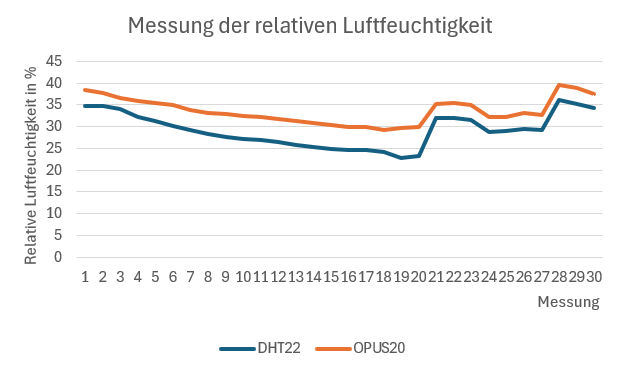
\includegraphics[width=9cm]{Sensor/DHT22/AbweichungFeuchte}
    \caption{Graph für Abweichung der Luftfeuchtigkeit}
    \label{fig:ABWH}
\end{figure}

\begin{figure}[H]
    \centering
    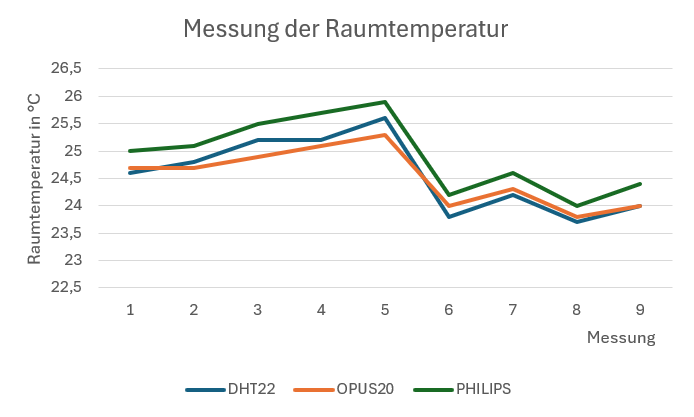
\includegraphics[width=9cm]{Sensor/DHT22/AbweichungTemperatur}
    \caption{Graph für Abweichung der Temperatur}
    \label{fig:ABWT}
\end{figure}

\begin{figure}[H]
    \centering
    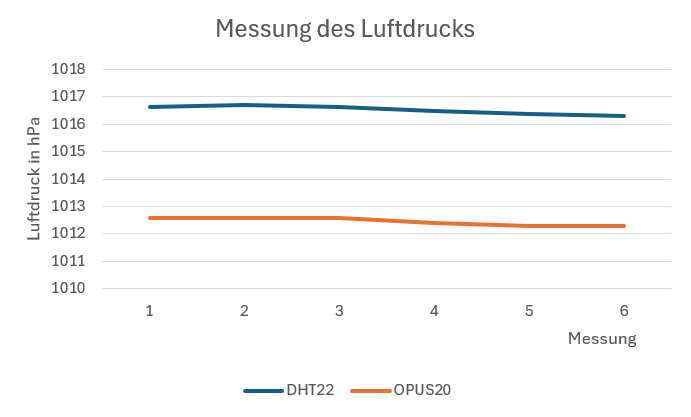
\includegraphics[width=9cm]{Sensor/DHT22/AbweichungDruck}
    \caption{Graph für Abweichung des Luftdrucks}
    \label{fig:ABWP}
\end{figure}